\clearpage
\section{関連研究}
分岐路で動的に経路を選択して移動する機能を有する視覚に基づくナビゲーションを,模倣学習により
獲得する手法はいくつか提案されている.
Felipeら\cite{codevilla2018endtoend}は視覚を入力とする模倣学習を,
左折や右折などの行動ごとにモデルを分けて行った.
このモデルを目標とする経路方向のベクトルによって切り替えることで,\figref{fig:felipe}に示す
経路選択が可能な視覚に基づく自律移動を行なっている.
\begin{figure}[htbp]
    \centering
     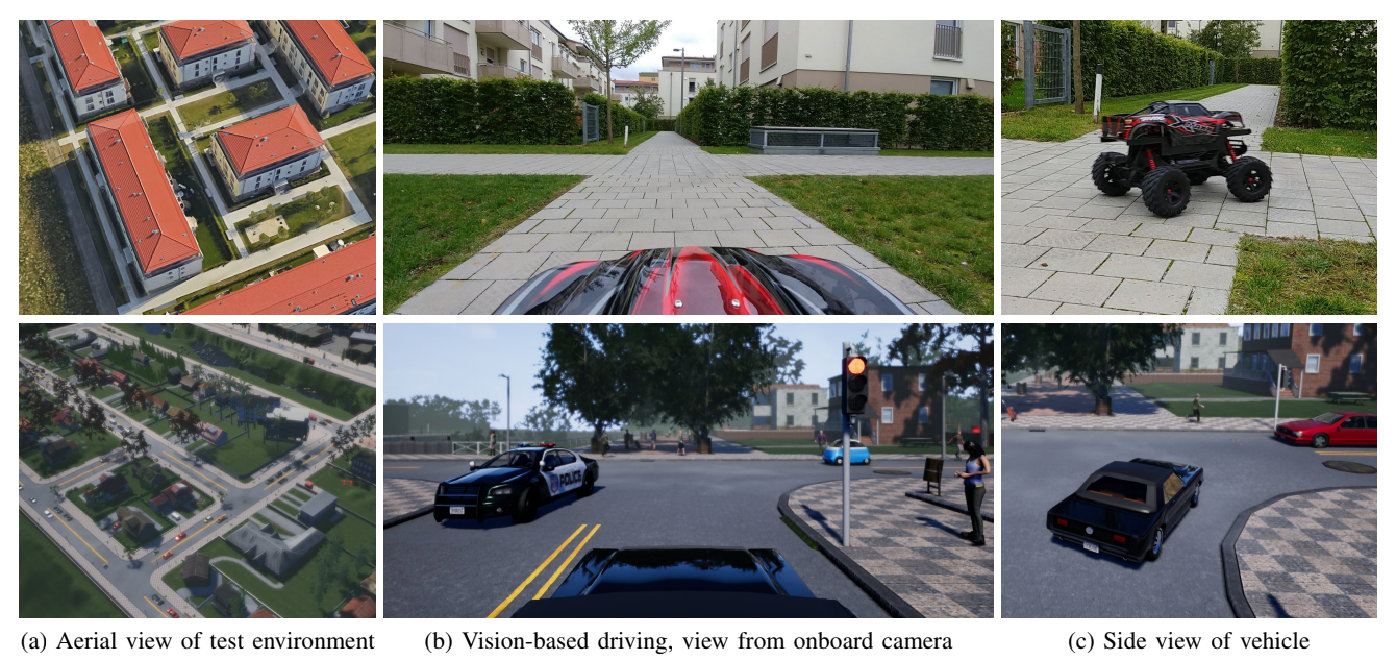
\includegraphics[width=120mm]{images/pdf/fleipe.pdf}
     \caption{End-to-end driving via conditional imitation learning (Quoted from\cite{codevilla2018endtoend})}
     \label{fig:felipe}
\end{figure}

Seiyaら\cite{seiya2018}は\figref{fig:seiya}に示すようにカメラ画像と目的地への方向を示すベクトルを入力,
ステアリングの角度を出力として模倣学習した.
これにより屋内外の分岐路で特定の経路が選択できることを確認している.
\begin{figure}[htbp]
    \centering
     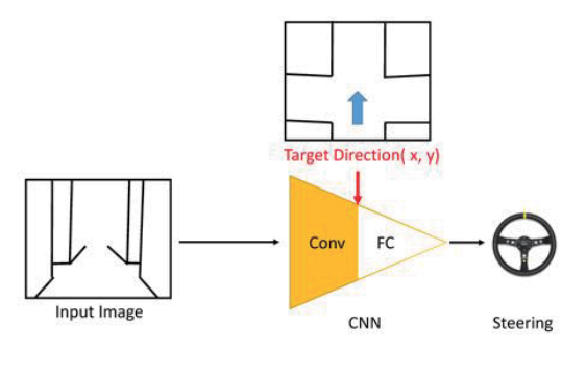
\includegraphics[width=100mm]{images/pdf/seiya.pdf}
     \caption{Overview of Seiya and others proposed method (Quoted from\cite{seiya2018})}
     \label{fig:seiya}
\end{figure}

これらの研究により,経路の情報を含めて模倣学習することで,経路選択が可能な
自律移動を獲得できることが確認されている.
\chapref{chap:path_select}ではこれらの
研究を参考に,岡田らの従来手法に対し,経路を選択する機能の追加を試みる.
\newpage
次に
任意の目的地に向けて移動が可能な視覚に基づくナビゲーションに
関連した研究について述べる.
Dhruvら\cite{shah2022lmnav}は,
大規模な事前学習モデルを用いて,自然言語指示と画像を組み合わせたナビゲーション行う手法を提案している.
この研究では,\figref{fig:lmnav}に示すように,
自然言語で指示されたランドマークを視覚によって検出し,これらのランドマークを経由して目的地への
ナビゲーションをしている.
% 目的地までランドマークを辿ることでナビゲーションを行う.
実験では,停車中の車,道路標識,曲がり角といった道路の特徴をランドマークとして利用している.

\begin{figure}[htbp]
    \centering
     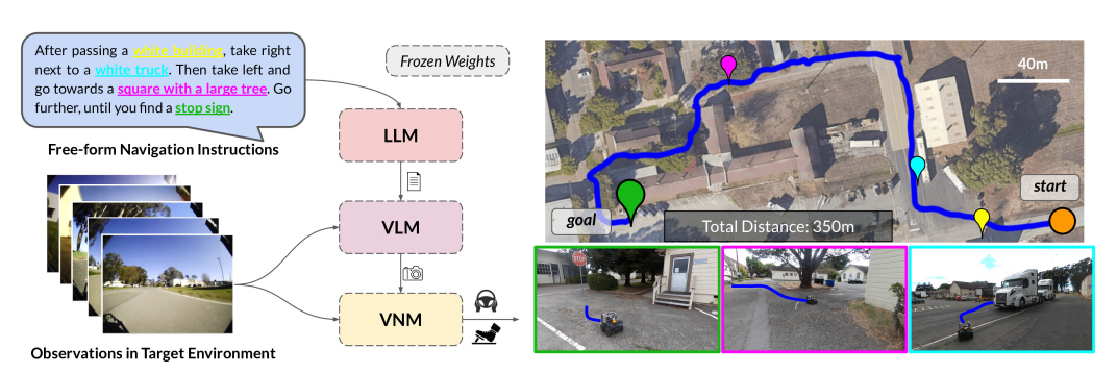
\includegraphics[width=120mm]{images/pdf/lmnav.pdf}
     \caption{Embodied instruction following with LM-Nav (Quoted from\cite{shah2022lmnav})}
     \label{fig:lmnav}
\end{figure}
\newpage
Miyamotoら\cite{miyamoto}は環境中のランドマークを含む\figref{fig:topo_meiji}に示すトポロジカルマップと,
\figref{fig:seg_meiji}に示すセマンティックセグメンテーションを用いた,視覚に基づくナビゲーション手法を提案している.
実験では,木などの植物や,建物,交差点などのランドマークを視覚によって検出し,
これらをトポロジカルマップ上での経路の決定に利用している.


\begin{figure}[h]
    \centering
     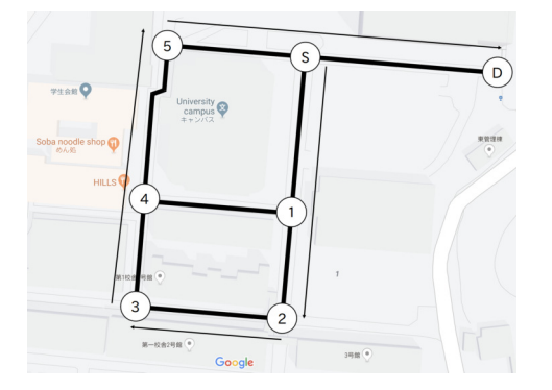
\includegraphics[height=60mm]{images/pdf/topo_meiji.pdf}
     \caption{Miyamoto and others used topological map (Quoted from\cite{miyamoto})}
     \label{fig:topo_meiji}
\end{figure}
\begin{figure}[h]
    \centering
     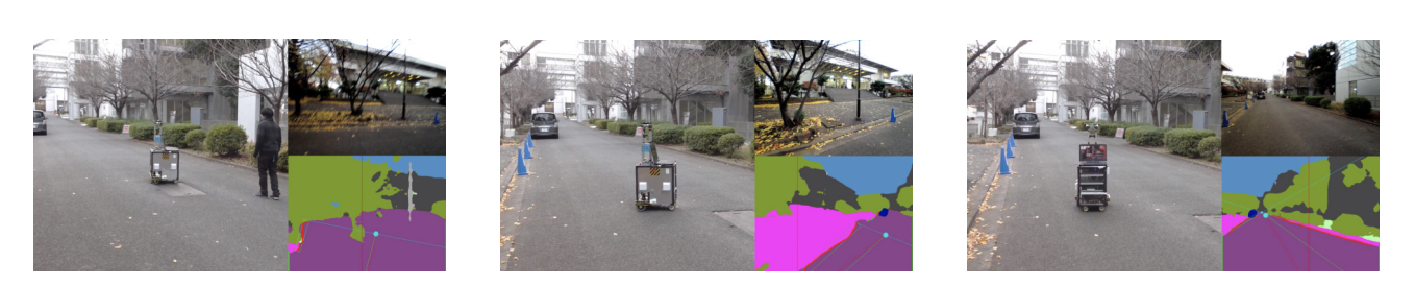
\includegraphics[width=120mm]{images/pdf/seg_meiji.pdf}
     \caption{Observation of robot behavior using semantic segmentation (Quoted from\cite{miyamoto})}
     \label{fig:seg_meiji}
\end{figure}

% これらの研究から,視覚に基づくナビゲーションにおいて,
% 設定した目的地まで自律移動するためには,標識や交差点といったランドマークの検出が
% 必要な要素であることが明らかになっている.
% 本論文では,分岐路において動的に経路を選択して移動することから
% 「分岐路」などの通路の特徴をランドマークとして扱い,これを視覚に基づいて検出する.

これらの研究では,視覚に基づくナビゲーションにおいて,目的地への自律移動に
標識や交差点といったランドマークを用いている.
本論文では,分岐路で動的な経路を選択した移動を行うことから,「分岐路」などの通路の特徴を
ランドマークとし,これを視覚に基づいて検出する.

% 手法では,補助的ではあるが,Global Navigation Satellite System(GNSS)や
% ホイールオドメトリといった情報を必要としている.
% センサ入力という観点で比較すると,\chapref{chap:scenario_vision}で述べるシステムは
% カメラ画像のみで目的地まで移動できるという違いがある.